\section{The Spatial Compiler}
\label{compiler}

When targeting FPGAs, the Spatial compiler provides source-to-source translations from applications in the Spatial language to synthesizable hardware descriptions in Chisel RTL~\cite{chisel}.
The output for CGRAs depends on the requirements of the hardware target. Host (CPU) code is generated in C++.
Spatial is designed to capture algorithms that are intended to run on reconfigurable architectures,
which gives rise to analyses and optimizations that are not used in software compilers.
In this section, we describe the compiler's intermediate representation and its key passes, as summarized in Figure~\ref{fig:compilerflow}.
Apart from Chisel generation, these passes are common to targeting both FPGAs and the Plasticine CGRA. Details of targeting Plasticine are discussed in prior work~\cite{plasticine}.

\begin{figure}
%%% trim = left, bottom, right, top
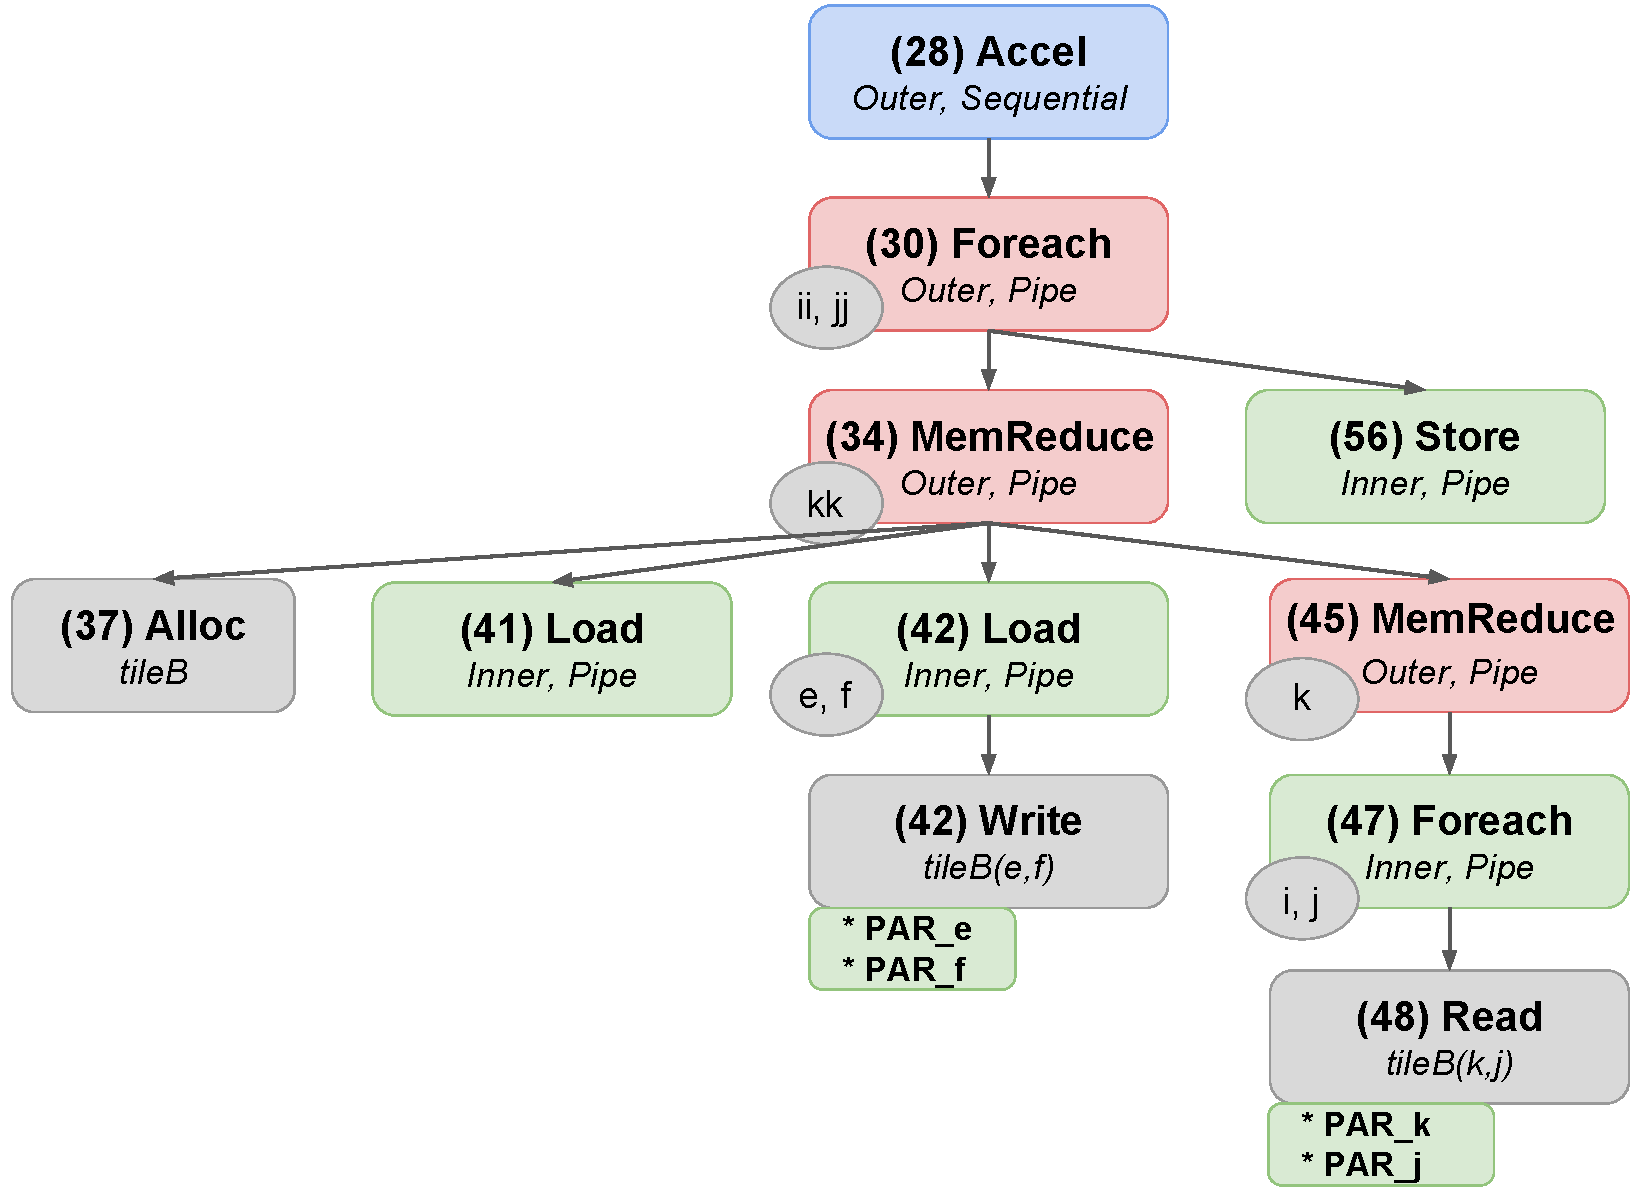
\includegraphics[clip, width=0.9\columnwidth]{figs/control_tree_gemm.pdf}
\vspace{-10pt}
\caption{The control/access tree for the \texttt{\small{SRAM tileB}} in the matrix multiply example in Figure~\ref{fig:matmult}.
%Control nodes are annotated with their level (outer versus inner), schedule, and loop iterator name. Memory access nodes are annotated with their parallelization factor.
\vspace{-5pt}
}
\label{fig:controlTree}
\end{figure}

\subsection{Intermediate Representation}

Spatial programs are internally represented in the compiler as a hierarchical dataflow graph (DFG).
Nodes in this graph represent control structures, data operations, and memory allocations, while edges represent data and effect dependencies.
Nesting of controllers directly translates to the hierarchy in the intermediate representation.
Design parameters are kept as graph metadata, such that they can be independently updated without changing the graph itself.


When discussing DFG transformations and optimizations, it is often useful to think about the graph as a controller/access tree. Figure~\ref{fig:controlTree} shows an example of one such controller tree for the memory {\texttt{\small{tileB}} in the Spatial code example in Figure~\ref{fig:matmult}. Note that transfers between on-chip and off-chip memory expand to a control node which linearly accesses the on-chip memory, in this case by iterators \texttt{e} and \texttt{f}.
This tree abstracts away most primitive operations, leaving only relevant controller hierarchy and the memory
accesses for a specific memory.


Within the acceleratable subset of Spatial, nodes are formally separated into three categories:
control nodes, memory allocation nodes, and primitive nodes.
Control nodes represent state machine structures like \texttt{\small{Foreach}} and \texttt{\small{Reduce}} described in Section~\ref{controls}.
Primitive nodes are operations which may consume, but never produce, control signals, including on-chip memory accesses.
Primitive nodes are further broken down into ``physical'' operations requiring resources and ``ephemeral'' operations which are only used for bookkeeping purposes in the compiler. For example, bit selects and grouping of words into structs require no hardware resources but are used to track necessary wires in the generated code.

% The nodes that compose the IR of Spatial provide the handles necessary to do a range of
% hardware optimizations that are specific to spatial architectures.  The combination of
% metadata associated with each node and the hierarchical structure AST that exposes relationships
% between primitives and control structures make it easy to do optimizations on the scheduling of
% controllers, buffering, banking, and duplication of memory elements, and comprehensive DSE over
% the provided parameter space with low latency.
% \subsection{DRAM Request Consolidation}
% In memory-bound applications, the only way to improve performance is to make better use
% of the available bandwidth.  It is well known that memory bandwidth asymptotically approaches the DRAM's peak bandwidth \todo{is this true?}
% as the size of each request increases.  This is because of how DRAM pays a penalty for activating and retiring
% lines of memory cells, and can return more data quickly when consecutive bursts are requested with the same command.

% Unfortunately, there are many applications where the programmer may opt to create logical tensors with
% relatively small leading dimensions and attempt to load multi-dimensional portions of the structure into on-chip SRAM
% without awareness of how this may thrash the DRAM's controllers in an inefficient way.  For example,
% the programmer may want to solve a multi-objective gradient descent problem that has many training points and very
% few objectives, hence creating a tall and skinny Y matrix.

% The compiler is able to recognize when the application will be sending out multiple requests to DRAM with
% consecutive addresses, and rewrite the controller to consolidate these into fewer, longer burst commands.
% This means that the user will get fully optimized DRAM requests and physical hardware without needing
% to rethink or change the semantics of the source code.

\subsection{Control Insertion}

To simplify reasoning about control signals, Spatial requires that control nodes do not contain both physical primitive nodes and other control nodes. The exception to this rule is conditional \texttt{\small{if}} statements, which can be used in the same scope as primitives as long as they contain no control nodes but conditionals themselves.
This requirement is satisfied by a DFG transformation which inserts \texttt{\small{DummyPipe}} control nodes around primitive logic in control bodies which also contain control nodes. The \texttt{\small{DummyPipe}} node is a bookkeeping control structure which is logically equivalent to a loop with exactly one iteration.
Thereafter, control nodes with primitive nodes are called ``inner'' control nodes, while controllers which contain other nested controllers are called ``outer'' nodes.

% For example, Figure~\ref{fig:matmult} contains some of these nodes. The Foreach in line 32 is an ``outer'' controller, which contains a memory allocation node for tileC
% (line 33) and another control node, \texttt{\small{MemReduce}} in line 38.  The \texttt{\small{Foreach}} in line 51 is an ``inner'' controller, as it contains
% only primitive nodes generated by the SRAM reads, multiplication, and SRAM store inlined on line 52.


\subsection{Controller Scheduling}
\label{scheduling}
After controller insertion, the compiler will then schedule the operations within each controller.
By default, the compiler will always attempt to pipeline loops regardless of nesting level.
The behavior of the compiler's scheduler can be overridden by the user using the directives listed in Table~\ref{t:syntaxTable}b.

Inner pipeline schedules are based on their initiation interval.
The compiler first collects resource initiation intervals for each primitive node in the given controller based on an internal, target-dependent lookup table.
Most primitive operations are pipelined for a resource initiation interval of 1.
The compiler then calculates all loop carried dependencies within the pipeline based on the dataflow graph.
For non-addressable memories, the total initiation interval is the maximum of path lengths between all dependent reads and the writes.
For addressable memories, the path length of loop carried dependencies is also multiplied by the difference in write and read addresses.
If the addresses are loop-independent, the initiation interval is the path length if they may be equal, and 1 if they are provably not equal. If the distance between the addresses cannot be determined statically, the initiation interval is infinite, meaning the loop must be run sequentially.
The total initiation interval is defined as the maximum of the initiation intervals of all loop carried dependencies and all resource initiation intervals.

The compiler also attempts to pipeline the bodies of outer control nodes in a similar manner, but computes dataflow scheduling in terms of inner control nodes and number of stages rather than primitive nodes and cycles. For example, the outer \texttt{\small{MemReduce}} in line 34 of Figure~\ref{fig:matmult} contains 4 sub-controllers: the load into \texttt{\small{tileA}} (line 41), the load into \texttt{\small{tileB}} (42), the inner \texttt{\small{MemReduce}} (45), and an reduction stage combining intermediate tiles (53). Based on data dependencies, the compiler infers that the two loads can be run in parallel, followed by the inner \texttt{\small{MemReduce}} and the tile reduction. It will also determine that multiple iterations of this outer loop can also be pipelined through these stages.

\subsection{Memory Analysis}
\label{memopts}

Loop parallelization only serves to improve performance if there is sufficient on-chip bandwidth to feed the duplicated computation.
Spatial's memory analysis banks and buffers on-chip memories to maximize this available on-chip read and write bandwidth.
Memory banking, also called data partitioning, is the process of dividing a memory's address space across multiple physical instances in order to create
additional ports for concurrent accesses within the same controller.
Partitioning is possible when the access patterns are statically predictable and guaranteed to never conflict access the same port/bank.
While a single port can be time multiplexed, this entirely negates the benefits of parallelization by increasing the whole pipeline's required initiation interval.
Note that while banking can trivially be achieved by memory duplication, Spatial aims to also minimize the total amount of memory resources.

Spatial leverages the memory partitioning strategy based on conflict polytope emptiness testing described by Wang et. al.~\cite{Wang_banking}. We extend this strategy by accounting for random access patterns and memory accesses across nested loops. Random accesses are modeled as additional dimensions in the conflict polytope as if they were additional loop iterators. Spatial minimizes the number of random access symbols used in this way by identifying affine combinations of random values. For example, an access to a memory at address $x$ and $x+1$ only requires one random variable, $x$, as the second is a predictable, affine function of the first.
Spatial also supports banking per dimension to account for cases where only some dimensions are accessed predictably.

Non-addressed memories like \texttt{\small{FIFOs}} and \texttt{\small{FILOs}} are modeled as addressed memories.
Each access to these memory types is represented as a linear access of all loop iterators around the memory access relative to the memory's definition. Spatial forbids parallelization of outer loops around non-addressed accesses, as this violates the guarantee of equivalent behavior to sequential execution.

To handle multiple pipelined accesses across stages within an outer loop, Spatial also automatically buffers on-chip memories.
Buffering creates multiple copies of the
same memory for maintaining versions of the data across overlapped loop iterations.
Without this optimization, pipeline parallel accesses to the same memory across different stages of a coarse-grain pipeline would not be able to run concurrently.
See Appendix~\ref{banking-appendix} for details on how both banking and buffering are computed.


For example, as shown in Figure~\ref{fig:controlTree}, \texttt{\small{tileB}} has two parallelized accesses, the load on line 42 and the read on line 48. If all (implicit and explicit) parallelization factors are set to 2, this corresponds to 4 accesses per loop. Spatial then builds the access polytope corresponding to all accesses in each loop, and determines the banking strategy that works for both loops. In this example, this means the SRAM will be banked such that each element within a 2x2 square will reside
in a different physical bank to allow fully parallel access. If the \texttt{\small{MemReduce}} on line 34 is pipelined, \texttt{\small{tileB}} will be double buffered to protect the reads (line 48) in one iteration of the outer loop
from the writes (line 42) in the next iteration.

\begin{figure}
\centering
\hspace{5pt}
\begin{tabular}{l}
\hline\hline
% function ReachingWrites:
%   input: $I_w$ $\rightarrow$ set of sets of writes
%   input: $I_r$ $\rightarrow$ set of sets of reads
%   $I'_w$ = $\emptyset$
%   $R$ = Flatten($I_r$)
%   for all $W$ in $I_w$:
%     $W'$ = {$w~\forall~w \in W$ s.t.
%             $\exists~r \in R$ s.t. MayPrecede($w$,$r$) $\vee~w \cap r \neq \emptyset$}
%     if $W' \neq \emptyset$: add $W'$ to $I'_w$
%   return $I_w'$
% end function

{\begin{lstlisting}[language=Pseudo,linewidth=0.98\columnwidth, mathescape=true]
function GroupAccesses:
   input: $A$ $\rightarrow$ set of reads or writes to $m$

   $G$ = $\emptyset$ set of sets of compatible accesses

   for all accesses $a$ in $A$:
      for all sets of accesses $g$ in $G$:
       if IComp($a$, $a'$) for all $a'$ in $g$ then
          add $a$ to $g$
          break
       else add {$a$} to $G$

   return $G$
end function

function ConfigureMemory:
   input: $A_r$ $\rightarrow$ set of reads of $m$
   input: $A_w$ $\rightarrow$ set of writes to $m$

   $G_r$ = GroupAccesses($A_r$)
   $G_w$ = GroupAccesses($A_w$)

   $I$ = $\emptyset$ set of memory instances

   for all read sets $R$ in $G_r$:
      $I_r$ = {$R$}
      $I_w$ = ReachingWrites($G_w$, $I_r$)
      $i$ = BankAndBuffer($I_r$, $I_w$)
      for each $inst$ in $I$:
         $I'_r$ = ReadSets[$inst$] + $R$
         $I'_w$ = ReachingWrites($G_w$, $I'_r$)
         if OComp($A_1$,$A_2$) $\forall A_1 \neq A_2 \in (G_w \cup I'_r)$ then:
            $i'$ = BankAndBuffer($I'_r$, $I'_w$)
            if Cost($i'$) < Cost($i$) + Cost($inst$) then:
               remove $inst$ from $I$
               add $i'$ to $I$
               break

      if $i$ has not been merged then add $i$ to $I$

   return I
end function
\end{lstlisting}}\\
\hline
\end{tabular}
\caption{Banking and buffering algorithm for calculating instances of on-chip memory $m$.}
\label{fig:bank_alg}
\end{figure}

Figure~\ref{fig:bank_alg} gives pseudocode for Spatial's algorithm to bank and buffer accesses to a given memory \emph{m} across loop nests. For each access $a$ to $m$, we first define an iteration domain $D$ for that access. This domain is the multi-dimensional space of possible values of all loop iterators for all loops which contain $a$ but which do not contain $m$.

We then group read and write accesses on $m$ into ``compatible'' sets which occur in parallel to the same physical port but which can be banked together (lines 1 -- 14).
Two accesses $a_1$ and $a_2$ within iteration domains $D_1$ and $D_2$
are banking compatible ($IComp$) if
\[ IComp(a_1,a_2) = \nexists~\vec{i} \in (D_1 \cup D_2) ~s.t.~a_1(\vec{i}) = r_2(\vec{i}) \]
where $a(i)$ is the multi-dimensional address corresponding to access $a$ for some vector of iterator values $i$.
This check can be implemented using a polytope emptiness test.

After grouping, each group could be directly mapped to a coherent ``instance'', or copy, of $m$.
However, this approach would typically use more resources than required. To minimize the total number of memory instances, we next greedily merge groups together (lines 25 -- 39). Merging is done when the cost of a merged instance is less than the cost of adding a separate, coherent instance for that group.
Two sets of accesses $A_1$ and $A_2$ allow merging ($OComp$) if
\[ OComp(A_1, A_2) = \nexists~ (a_1 \in A_1, a_2 \in A_2) ~s.t. \]
\[  LCA(a_1, a_2) \in Parallel \cup (Pipe \cap Inner) \]
where \emph{Parallel}, \emph{Pipe}, and \emph{Inner} are the set of Parallel, pipelined, and inner controllers in the program, respectively.
If this condition holds, all accesses between the two instances either occur sequentially or occur as part of a coarse-grain pipeline. Sequential accesses can be time multiplexed, while pipelined accesses are buffered.

\emph{ReachingWrites} returns all writes in each set which may be visible to any read in the given sets of reads. Visibility is possible if the write may be executed before the read and may have an overlapping address space.

The \emph{BankAndBuffer} function produces a single memory instance from memory reads and writes.
Here, each set of accesses is a set of parallel reads or writes to a single port of the memory instance.
Accesses in different sets are guaranteed not to occur to the same port at the same time.
Therefore, a common banking strategy is found which has no bank conflicts for any set of accesses.
This banking strategy is found using iterative polytope emptiness testing as described by Wang et. al.~\cite{Wang_banking}.
A separate emptiness test is run for each set of parallel accesses for each proposed strategy.

The required buffer depth \emph{d} for a pair of accesses $a_1$ and $a_2$ to $m$ is computed as
\[
d(a_1, a_2) = \left\{\begin{matrix} 1 & LCA(a_1, a_2) \in Seq \cup Stream \\ dist(a_1,a_2) & LCA(a_1,a_2) \in Pipe \end{matrix}\right.
\]
where \emph{dist} is the minimum of the depth of the LCA and the dataflow distance of the two direct children of the LCA which contain $a_1$ and $a_2$. \emph{Seq}, \emph{Stream}, and \emph{Pipe} are the set of sequential, streaming, and pipelined controllers, respectively. Buffering addressable memories across streaming accesses is currently unsupported.
The depth of a set of reads $R$ and writes $W$ is then
\[ Depth(R,W) = max\{ d(w,a)~\forall ~(w,a) \in W \times (W\cup R) \} \]

The port of each access within a buffer is determined from the relative distances between all buffered accesses.
Spatial requires that no more than one coarse-grained controller or streaming controller is part of a merged instance.
The final output of the greedy search is a set of required physical memory instances for memory \emph{m}.



\subsection{Area and Runtime Estimation}
\label{sec:modeling}
In this section, we describe our modeling methodology. Our models account for the various
design parameters for each Spatial node, as well as optimizations done by low-level logic
synthesis tools in order to accurately estimate resource usage.

\subsection{Modeling Considerations}
\label{ss:modeling-con}
%\gist{Low-level tools do fancy optimizations which estimator should be aware of.
%  Examples: LUT packing, logic duplication, using BRAMs for large delay lines,
%unavailable LUTs etc. Also, certain device architecture features play a significant role}
The resource requirements of a given application implemented on an FPGA depend both on the target device and on the toolchain.
Heterogeneity in the FPGA fabric, use of FPGA resources for routing, and other low-level optimizations performed by logic
synthesis tools often have a significant impact on the total resource consumption of a design. Since these factors reflect
the physical layout of computation on the device after placement and routing, they are not captured directly in the application's dataflow graph.
We identify and account for the following factors:
%\begin{itemize}

\paragraph{LUT and register packing} Basic compute units in FPGAs are typically composed of a lookup table (LUT), and a small number of single bit multiplexers, registers, and full adders.
  Modern FPGA LUTs support up to 8-input binary functions but are often implemented using a pair of smaller LUTs~\cite{stratixv,virtex7}.
  When these LUTs can be configured and used independently, vendor placement tools attempt to ``pack'' multiple small functions into a single 8-input unit.
  LUT packing can have a significant impact on design resource requirements.
  In our experiments, we are able to pack about 80\% of the functions in each design in pairs, decreasing the number of used LUTs by about 40\%.

\paragraph{Routing Resources} Logic synthesis tools require a significant amount of resources to establish static routing connections
between two design points (e.g., a multiplier and a block RAM) which fit in the path's clock period. While FPGAs have dedicated routing resources,
logic synthesis tools may have the option to use LUTs for routing. These LUTs may then be unavailable to be used for ``real'' compute.
In our designs, ``route-through'' LUTs typically account for about 10\% of the total number of used LUTs.


\paragraph{Logic duplication} Logic synthesis tools often duplicate resources such as block RAMs
and registers to avoid routing congestion and to decrease fan out. While duplicated registers typically
encompass around 5\% of the total number of registers required in our designs, we found that block RAM
duplication can increase RAM utilization by 10 to 100\%, depending on the complexity of the design.


\paragraph{Unavailable resources} FPGA resources are typically organized in a hierarchy, such as Altera's Logic Array Block structure (10 LUTs)
and Xilinx's Slice structure (4 LUTs). Such organizations impose mapping constraints which can lead to
resources that are rendered unusable. In our experiments, the number of unusable LUTs made up only about 4\% of the design's total LUT usage.
%\end{itemize}
%\todo{Need to figure out how to say this.} We focus on one Altera device in this paper, the Stratix V.
%ALMs in the Stratix V have 4 registers. We experimentally found that in most designs, just over 50 percent
%of the registers in each ALM is used. Thus, we use a simple model where we assume registers do not
%contribute to the ALM count unless they number over 2x the number of ALMs used to implement logic.
%(packed lut count) + max(0, regs/2 - (packed lut count))

\subsection{Methodology}
In order to model runtime and resource requirements of Spatial designs, we first need an estimate of the area requirements and
propagation delay of every Spatial node. Area requirements include the number of digital signal processing
units (DSPs), device block RAMs, LUTs, and registers that each template requires. To facilitate LUT packing estimation,
we split template LUT resource requirements into the number of ``packable'' and ``unpackable'' LUTs required.
%For templates with documented implementations such as floating point operations \cite{fp-altera}, we gather resource and cycle data in part by summarizing IP core documentation. However, these user manuals typically do not give resource usage breakdowns at the binary function level.
We obtain characterization data by synthesizing multiple instances of each template instantiated for combinations of its parameters as given in Table~\ref{t-hwtemplates}.
Using this data, we create analytical models of each Spatial nodes's resource requirements and cycle counts for
a predefined fabric clock. The area and cycle count of controller templates are modeled as functions of the latencies of the nodes contained within them.
The total cycle count for a \emph{MetaPipe}, for example, is modeled using the recursive function
\begin{displaymath}
(N-1)\max(cycles(n) | n \in nodes) + \sum_{n \in nodes} cycles(n)
\end{displaymath}
where \emph{N} is the number of iterations of the \emph{MetaPipe} and \emph{nodes} is the set of nodes contained in the \emph{MetaPipe}.

Most templates require about six synthesized designs to characterize their resource and area usage as a function of their parameters. Note that these models include estimates of off-chip memory access latency as a function of the
number and length of memory commands, as well as contention due to competing accessors. Since template models are application-independent, each needs only be characterized once for a given target device and logic synthesis toolchain. The synthesis times required to model templates can therefore be amortized over many applications.
%We show a subset of the template models used in our experiments in Table~\ref{table:benchmarks}.
%\note{not sure I understand this. Which part is app-independent. Presumably the way to explore the space will dependt on the application. Is this only for the device models? }

Using these models, we run a pair of analysis passes over the application's intermediate representation to estimate design cycle counts and area requirements.

\subsubsection{Cycle Count Estimation}
In the first analysis pass, we estimate the total runtime of the design on the FPGA.
Since the Spatial intermediate representation is hierarchical in nature, this pass is done recursively.
The total runtime of \emph{MetaPipe} and \emph{Sequential} nodes is calculated first by determining
the runtime of all controller nodes contained within them. The total propagation delay of a single
iteration of a \emph{Pipe} is the length of the body's critical path, calculated using a depth first
search of the body's subgraph and the propagation delay of all primitive nodes within the graph.
Input dataset sizes, given as user annotations in the high-level program, are used by the analysis pass
along with tiling factors to determine the iteration counts for each controller template.
Iteration counts are then used to calculate the total runtime of the respective controller nodes. %using the equations given in Table~\ref{table:benchmarks}.


\subsubsection{Area Estimation}
Since the FPGA resource utilization of a design is sensitive to factors that are not directly captured
in the design's dataflow graph, we adopt a hybrid approach in our area analysis.

We first estimate the area of the design by counting the resource
requirements of each node using their pre-characterized area models. In \emph{Pipe} bodies, we also
estimate the resources required for delaying signals. This is done by recursively calculating the
propagation delay of every path to each node using depth first search. Paths with slack relative to
the critical path to that node require their width (in bits) multiplied by the slack delay resources.
Delays over a synthesis tool-specific threshold are modeled as block RAMs.
Otherwise, they are modeled as registers. Note that this estimation assumes ASAP scheduling.

We model LUT routing usage, register duplication, and unavailable LUTs using a set of small artificial
neural networks implemented using the Encog machine learning library~\cite{encog}.
Each network has three fully connected layers with eleven input nodes, six hidden layer nodes, and a single output node. We chose to use
three layer neural networks as they have been proven to be capable of fitting a wide number of function classes with arbitrary precision, including polynomial functions of any order~\cite{science}.
One network is trained
for each factor on a common set of 200 design samples with varying levels of resource usage to give a representative sampling of the space. Choosing the correct
network parameters to obtain the lowest model error is typically challenging, but in our experiments we found that above four nodes in the hidden layer,
the exact number of hidden layer nodes made little difference.
Duplicated block RAMs are estimated as a linear function of the number of routing LUTs, as we found that this gave the best estimate of design routing complexity in practice. This linear function was fit using the same data used to train the neural networks. Like the template models, these neural networks are application independent and only need to be trained once for a given target device and toolchain.

We use the raw resource counts as an input to each of our neural networks to obtain global estimates for routing LUTs,
duplicated registers, and unavailable LUTs. We estimate the number of duplicated block RAMs using the routing LUTs.
These estimates are then added to the raw resource counts to obtain a pre-packing resource estimate. For the purposes
of LUT packing, we assume routing LUTs are always packable.

Lastly, we model LUT packing using the simple assumption that all packable LUTs will be packed. The target device
in our experiments supports pairwise LUT packing, so we estimate the number of compute units used for logic as
the number of unpackable LUTs plus the number of packable LUTs divided by two. We assume that each compute unit
will use two registers on average. We model any registers unaccounted for by logic compute units as requiring
compute units with two registers each. This gives us the final estimation for LUTs, DSPs, and BRAM.

%To account for resources utilized by nodes in the dataflow graph, we then perform a detailed characterization of all primitive nodes
%in DHDL and use the data to count the resources required to implement the datapath.

%We use a simple model for LUT packing, where we assume that pairs of LUTs which
%can be packed are packed.
%Table \todo{Table with control, memory, and mem generator templates as functions + description of what each variable is - should have four columns(?): node name, area function, and cycle function, and variable description?} gives examples of the resource usage and cycle latency of memory, controller, and memory command generator templates as functions of their respective parameters.
%We model each of the factors listed in section~\ref{ss:modeling-con} using a two layer artificial neural networks

%We use the Encog machine learning library~\cite{encog} to implement our neural network.

\subsection{Design space exploration}
Our design space exploration tool uses the resource and cycle count estimates
to explore the space of designs described by the parameters in Table~\ref{t-hwtemplates}.
As we are dealing with large design spaces on the order of millions of points even for small benchmarks,
we prune invalid and suboptimal points in the search space using a few simple heuristics:
\begin{itemize}
  \item Parallelization factors considered are integer divisors of the respective iteration counts. We use this pruning strategy because non-divisor factors create edge cases which require additional modulus operations. These operations can significantly increase the latency and area of address calculation, typically making them poor design parameter choices \cite{raghus-paper}.
  \item Tile sizes considered are divisors of the dimensions of the annotated data size. Similar to parallelization factors, tile sizes with edge cases are usually suboptimal as they increase load and store area and latency with additional indexing logic.
  \item Automatic banking of on-chip memories eliminates the memory banks as an independent variable. This prunes a large set of suboptimal design points where on-chip memory bandwidth requirements do not match the amount of parallelization.
  \item The total size of each local memory is limited to a fixed maximum value.
\end{itemize}

These heuristics defines a ``legal'' subspace of the total design space.
In our experiments, we randomly generate estimates for up to $75,000$ legal
points to give a representative view of the entire design space. We immediately
discard illegal points.



\subsection{Design Space Exploration}
\label{dse}
The scheduling and memory banking options identified by the compiler, together with loop parallelization and tile size parameters, forms a design space for the application.
The design tuning pass is an optional compiler pass which allows for fast exploration of this design space in order to make area/runtime design tradeoffs.
When design tuning is enabled, it repeatedly picks design points and evaluates them by rerunning the control scheduling, memory analysis, and estimation analysis passes. The output from this search is a single set of parameters from the Pareto frontier.

Unfortunately, application design spaces tend to be extremely large, and exhaustive search on an entire space is often infeasible. Of the benchmarks discussed in Section~\ref{evaluation},
only BlackScholes has a relatively small space of about $80,000$ points. While this space can be explored exhaustively by Spatial in a few minutes, other spaces are much larger, spanning $10^6$ to $10^{10}$ points and
taking hours or days to exhaustively search. For example, even with the few explicit design parameters exposed in the code in Figure~\ref{fig:matmult}, when combined with implicit pipelining and parallelization parameters, this code already has about $2.6\times10^8$ potential designs.
DHDL~\cite{dhdl} employed random search after heuristic pruning, reducing the total space by two to three orders of magnitude. However, this approach has high variance on larger design spaces and may inadvertently prune desirable points.

To reduce the variance on larger design spaces, Spatial's design space exploration flow integrates an active learning-based autotuner called HyperMapper~\cite{Bodin2016:PACT16,NardiBSVDK17,Saeedi_ICRA_2017}.
HyperMapper is a multi-objective derivative-free optimizer (DFO), and has already been demonstrated on the SLAMBench benchmarking framework \cite{nardi2015introducing}.
HyperMapper creates a surrogate model using a Random Forest regressor, and predicts the performance over the parameter space. This regressor is initially built using only few hundred random design point samples and is iteratively refined in subsequent active learning steps.

\subsection{Unrolling}
Following selection of values for design parameters, Spatial finalizes these parameters in a single graph transformation which unrolls loops and duplicates memories as determined by prior analysis passes.
\texttt{Reduce} and \texttt{MemReduce} patterns are also lowered into their imperative implementations, with hardware reduction trees instantiated from the given reduction function.
The two \texttt{MemReduce} loops in Figure~\ref{fig:matmult}, for example, will each be lowered into unrolled \texttt{Foreach} loops with explicitly banked memory accesses and explicitly duplicated multiply operations. The corresponding reduction across tiles (lines 52~--~53) are lowered into a second stage of the \texttt{Foreach} with explicit reduction trees matching the loop parallelization.

\subsection{Retiming}
After unrolling, the compiler retimes each inner pipeline to make sure data and control signals properly line up and ensure that the target clock frequency can be met.
To do this, the compiler orders primitive operations within each pipeline based on effect and dataflow order.
This ordering is calculated using a reverse depth first search along data and effect dependencies.
A second forward depth first search is then used to minimize delays in reduction cycles.
Based on this ordering, the compiler then inserts pipeline and delay line registers based on lookup tables which map each primitive node to an associated latency. Dependent nodes which have less than a full cycle of delay are kept as combinational operations, with a register only being inserted after the last operation.
This register insertion maximizes the achievable clock frequency for this controller while also minimizing the required initiation interval.



\begin{table*}

\fontsize{8}{9}\selectfont
\begin{tabular}{m{36pt} m{56pt} m{32pt} l d{3.0} d{6.0} d{4.0} d{4.0} d{4.1} }
\ml{}                                                           & \ml{}           &\ml{}          & \ml{}                & \mc{LOC}    & \mc{LUTs}         & \mc{BRAM}         & \mc{DSPs}         & \mc{Time (ms)} \\ \toprule
\ml{Benchmark}                                                  & \ml{Data Sizes} &\ml{DSE size}  & \ml{\emph{Capacity}} & \mc{---}    & 914400            & 1680              & 5640              & \mc{---} \\
\midrule

% \multirow{3}{*}{
% \hspace{-8pt}\begin{tabular}{l}
% \bf{AES} \\
% Encryption \\
% \end{tabular}
% }                                                               &
% \multirow{3}{*}{32kB data }
%                                                                 & SDAccel         & 333                  & 338305      & 589               & 0                 & 2.23 \\
%                                                                 &                 & Spatial              & 150         & 600027            & 442               & 9                 & 14.45 \\
%                                                                 &                 & \ml{Relative}        & \mc{54.8\%} & \mc{0.56$\times$} & \mc{1.33$\times$} & \mc{1.33$\times$} & \mc{0.15$\times$} \\ \midrule

\multirow{3}{*}{
\hspace{-8pt}\begin{tabular}{l}
\bf{BS} \\
Black-Scholes \\
option pricing \\
\end{tabular}
}                                                               &
\multirow{3}{*}{ 960,000 options }
& \multirow{3}{*}{ $7.7\times 10^4$ }
                                                                & SDAccel         & 175   & 363368      & 550  & 290 & 6.18 \\
                                              &&                & Spatial         & 93    & 698885      & 493  & 945 & 3.79 \\
                                              &                 &                 & \ml{Improv.} & \mc{46.8\%} & \mc{0.52$\times$} & \mc{1.12$\times$} & \mc{0.31$\times$} & \mc{1.63$\times$} \\ \midrule

\multirow{3}{*}{
\hspace{-8pt}\begin{tabular}{l}
\bf{GDA} \\
Gaussian \\
discrimination \\
\end{tabular}
}                                                               &
\multirow{3}{*}{
\hspace{-8pt}\begin{tabular}{l}
1024 rows \\
96 dimensions \\
\end{tabular}
} & \multirow{3}{*}{ $3.0\times 10^{10}$ }
                                                                & SDAccel          & 73    & 356857      & 594   & 108   & 10.75 \\
                                              &&                 & Spatial          & 64    & 378130      & 858   & 216   & 1.27  \\
                                              &&                 & \ml{Improv.} & \mc{12.3\%} & \mc{0.94$\times$} & \mc{0.69$\times$} & \mc{0.50$\times$} & \mc{8.48$\times$} \\ \midrule


\multirow{3}{*}{
\hspace{-8pt}\begin{tabular}{l}
\bf{GEMM} \\
Matrix \\
multiply \\
\end{tabular}
}                                                               &
\multirow{3}{*}{
\hspace{-8pt}\begin{tabular}{l}
A: 1024$\times$1024 \\
B: 1024$\times$1024 \\
\end{tabular}
}
& \multirow{3}{*}{ $2.6\times 10^8$ }
                                                                & SDAccel          & 110         & 341894            & 674               & 206                & 1207.26 \\
                                              &&                 & Spatial          & 44          & 426295            & 500               & 798               & 878.45 \\
                                              &&                 & \ml{Improv.} & \mc{60.0\%} & \mc{0.80$\times$} & \mc{1.35$\times$} & \mc{0.26$\times$} & \mc{1.37$\times$} \\ \midrule


\multirow{3}{*}{
\hspace{-8pt}\begin{tabular}{l}
\bf{KMeans} \\
K-Means \\
clustering\\
\end{tabular}
}                                                               &
\multirow{3}{*}{
\hspace{-8pt}\begin{tabular}{l}
200 iterations \\
320$\times$32 points \\
\end{tabular}
}
& \multirow{3}{*}{ $2.1\times 10^6$ }
                                                                & SDAccel          & 146         & 356382            & 657               & 539               & 73.04 \\
                                              &&                 & Spatial          & 81          & 369348            & 453               & 105                & 53.25 \\
                                              &&                 & \ml{Improv.} & \mc{44.5\%} & \mc{0.96$\times$} & \mc{1.45$\times$} & \mc{5.13$\times$} & \mc{1.37$\times$} \\ \midrule




\multirow{3}{*}{
\hspace{-8pt}\begin{tabular}{l}
\bf{PageRank} \\
Node ranking \\
\end{tabular}
}                                                               &
\multirow{3}{*}{
\hspace{-8pt}\begin{tabular}{l}
DIMACS10 \\
Chesapeake \\
10000 iterations \\
\end{tabular}
}
& \multirow{3}{*}{ $4.1\times 10^3$ }
                                                                & SDAccel          & 112         & 337102            & 549               & 17                & 2041.62 \\
                                              &&                 & Spatial          & 77          & 418128            & 862               & 81                & 587.35 \\
                                              &&                 & \ml{Improv.} & \mc{31.2\%} & \mc{0.81$\times$} & \mc{0.64$\times$} & \mc{0.21$\times$} & \mc{3.48$\times$} \\ \midrule


% \multirow{3}{*}{
% \hspace{-8pt}\begin{tabular}{l}
% \bf{Sobel} \\
% Image edge detection \\
% \end{tabular}
% }                                                               &
% \multirow{3}{*}{512$\times$512 bmp}
%                                                                & SDAccel         & 90                   & 341100      & 560               & 0                 & 0.19 \\
%                                                                &                 & Spatial              & 50          & 514885            & 574               & 177               & 20.74 \\
%                                                                &                 & \ml{Improv.}        & \mc{44.4\%} & \mc{0.66$\times$} & \mc{0.98$\times$} & \mc{0.07$\times$} & \mc{0.01$\times$} \\ \midrule

\multirow{3}{*}{
\hspace{-8pt}\begin{tabular}{l}
\bf{SW} \\
DNA \\
alignment \\
\end{tabular}
}                                                               &
\multirow{3}{*}{256 base pairs}
& \multirow{3}{*}{ $2.1\times 10^6$ }
                                                                & SDAccel           & 240         & 541617            & 547               & 12                & 8.67 \\
                                              &&                 & Spatial           & 82          & 330063            & 470               & 9                 & 0.61 \\
                                              &&                 & \ml{Improv.}  & \mc{65.8\%} & \mc{1.64$\times$} & \mc{1.16$\times$} & \mc{1.33$\times$} & \mc{14.15$\times$} \\ \midrule


\multirow{3}{*}{
\hspace{-8pt}\begin{tabular}{l}
\bf{TQ6} \\
TPC-H Q6 \\
\end{tabular}
}                                                               &
\multirow{3}{*}{6,400,000 records}
& \multirow{3}{*}{ $3.5\times 10^9$ }
                                                                & SDAccel          & 74          & 356978            & 548               & 15                & 18.61 \\
                                              &&                 & Spatial          & 48          & 472868            & 574               & 393               & 13.97 \\
                                              &&                 & \ml{Improv.} & \mc{35.1\%} & \mc{0.75$\times$} & \mc{0.95$\times$} & \mc{0.04$\times$} & \mc{1.33$\times$} \\


\midrule
\ml{Average}                                  &&                 & \ml{Improv.} & \mc{42.3\%} & \mc{0.87$\times$} & \mc{1.01$\times$} & \mc{0.42$\times$} & \mc{2.90$  \times$} \\

\bottomrule
\end{tabular}

\caption{Number of lines of code (LOC), area utilization, and runtime comparisons between SDAccel and Spatial on a single VU9P FPGA.
For reference, the first row lists the total number of FPGA resources available. LOC improvements are percent improvements from SDAccel. The remaining improvement factors are calculated as $(SDAccel / Spatial)$.}
\label{t:hls_comp}
\end{table*}


\subsection{Code Generation}
Prior to code generation, the compiler first allocates register names for every \texttt{\small{ArgIn}}, \texttt{\small{ArgOut}}, and \texttt{\small{HostIO}}.
In the final pass over the IR, the code generator then instantiates hardware modules from a library of custom, parameterized RTL templates written in Chisel and infers and generates the logic required to stitch them together.  These templates include state machines that manage communication between the various control structures and primitives in the application, as well as the banked and buffered memory structures and efficient arithmetic operations.  Finally, all generated hardware is wrapped in a target-specific, parameterized Chisel module that arbitrates off-chip accesses from the accelerator with the peripheral devices on the target FPGA.
